\chapter{Technologie tvorby}
\label{4-technologie}

\section{QGIS}

QGIS je profesionální geografický informační systém.
Software je zdarma ke stáhnutí a je tzv. open-source (zdrojový kód je veřejně).
Zdrojový kód je publikován na GitHubu \footnote{webová služba podporující vývoj softwaru za pomoci verzovacího nástroje Git}
a vývojář softwaru může být kdokoliv, avšak potvrzovat a kontrolovat změny můžou jen ověření
přispěvatelé.

QGIS je oficiálním projektem nadace OSGeo (Open Source Geospatial Foundation), což je nevládní 
nezisková organizace, jejíž cílem je podporovat a prosazovat společný vývoj otevřených geoinformačních
technologií. Běží na operačních systémech Linux, Unix, Mac OSX, Windows a Android a podporuje
řadu vektorových, rastrových a databázových formátů.

Kromě desktop verze QGISu existuje i QGIS Server, který umožňuje publikovat projekty a vrstvy
QGIS jako služby WMS, WMTS, WFS a WCS kompatibilní s OGC (Open Geospatial Consortium - mezinárodní standardizační organizace
o geoprostorových datech a službách).

\begin{figure}[H] \centering
    
\includegraphics[width=64pt]{./pictures/qgis-logo.png}
    \caption[Logo QGISu]{Logo QGISu \cite{qgis}}
	\label{fig:qgis-logo}                                
\end{figure}

\section{Python}
Python je moderní, dynamický, skriptovací programovací jazyk s veřejným zdrojovým kódem. 
Je snadný na naučení, lehko čitelný a v současné době velmi populární. Tento programovací jazyk využívají
softwaroví inženýři, matematici, datovi analytici, vědci, účetní a síťoví inženýři.
Dokonce kvůli jednoduchosti tohoto jazyka ho využívají i děti na základních školách.

Důvodů, proč je tento programovací jazyk tak populární, je mnoho. Python je vyšší programovací jazyk,
což znamená lépší srozumitelnost než nižších programovacích jazyků a programy zapsané
ve vyšších jazycích jsou obvykle kratší a lépe čitelné.  Další důvodem je multiplatformovost,
což znamená, že se můžou Pythoní aplikace sestavit a běžet na různých platformách jako 
Windows, Mac či Linux. Komunita Pythonu je obrovská, což je další výhodou tohoto jazyka.
Například jenom v Čechách je mnoho skupin na různých sociálních sítích.
Python má také spoustu knihoven, frameworků a nástrojů, které lidem usnadňují programování.

Podporuje různá programovací paradigmata
\footnote{základní programovací styl, který se liší v pojmech a abstrakcích,
které tvoří jednotlivé prvky programu, a krocích, ze kterých se výpočet skládá  
- objektově orientované, imperativní, procedurální nebo funkcionální \cite{wikipedia-paradigma}} 
jako například objektově orientované, imperativní, procedurální nebo funkcionální.

\begin{figure}[H] \centering
    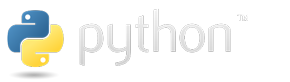
\includegraphics[width=260pt]{./pictures/python-logo.png}
    \caption[Logo Pythonu]{Logo Pythonu \cite{python}}
	\label{fig:python-logo}                                
\end{figure} 

\section{PyQt5}

\begin{figure}[H] \centering
    
\includegraphics[width=400pt]{./pictures/pyqt.png}
    \caption[Schéma PyQt5 Pythonu]{Schéma PyQt5}
	\label{fig:pyqt}                                
\end{figure} 